\subsection{Meldeprint}
%Der Hardwareaufbau des Meldeprints wird in diesem Kapitel zuerst grob beschrieben, anschliessend wird die Schaltung weiter aufgeteilt und jeder Bereich einzeln erläutert.
Der Meldeprint hat zur Aufgabe die von den einzelnen Panels übertragenen Informationen zu empfangen und diese auszuwerten. Er entscheidet, ob ein Panel fehlerhaft ist und zeigt dieses auf einem Display an. Der Meldeprint ist grundlegend aufgeteilt in die folgenden Schaltungsteile: Speisung, Mikrocontroller, Powerline Transceiver sowie Bedienung und Ausgabe. Diese einzelnen Bereiche sind in der Abbildung \ref{fig::HardKonzept} ersichtlich. Das Layout sowie das Schema der Platine sind im Anhang \ref{Layout_Melderpint} und \ref{Schema_Melderpint} angefügt.

\begin{figure}[h]
	\centering
	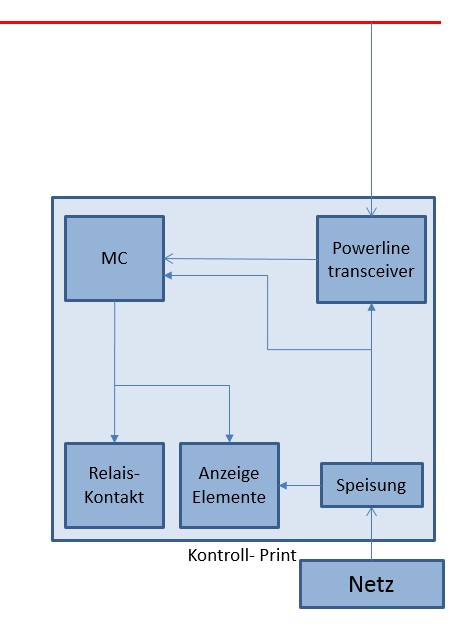
\includegraphics[width=0.5\textwidth]{konzept_melde.PNG}
	\caption{Grobkonzept des Meldeprints}
	\label{fig::HardKonzept}	
\end{figure}

In der Abbildung \ref{fig::HardKonzept} ist das Grundkonzept des Meldeprints zu sehen. Es zeigt das Zusammenspiel zwischen der Speisung, dem Powerline-Transceiver, Microkontroller und den Anzeige- respekive Ausgabeelementen.

\subsubsection{Speisung}
Als Speisung wird ein 230V-AC/DC-Netzgerät genommen. Dieses wandelt die Spannung in 24V-DC um welche wiederum mit zwei weiteren DC/DC-Wandlern in 12V für die Speisung des Mikrocontrollers und des Powerline Transceivers respektive 5V für die Logik Schaltung. Das 24V-AC/DC-Netzteil wurde gewählt da ein solches bereits vorhanden war und diese Spannung im Eingangsspannungsbereich der meisten DC/DC-Wandler liegt und so immer noch eine hohe Flexibilität in der Wahl dieser erlaubt. Für die DC/DC-Wandler wurden 2 Traco Power Step-Down Converter gewählt da diese keine externe Beschaltung benötigen und einen Wirkungsgrad grösser als 90 Prozent haben.

\subsubsection{Mikrocontroller}
Es wurde ein Arduino UNO als Mikrocontroller eingesetzt. Der UNO wurde gewählt, da dieser die benötigte Anzahl Ports besitzt und über einen genügend grossen Speicherplatz verfügt. Ein weiterer Vorteil waren die bereits angesammelten Fachkenntnisse in der Bedienung durch das Modul mc1, welche den Aufbau erleichterten.

Der Mikrocontroller regelt das Empfangen der Informationen der einzelnen Solarpanels sowie das Auswerten von diesen in begrifflich der Erkennung von Übertragungsfehlern. Er hat die Aufgabe die empfangenen Daten in einer sinnvollen Struktur abzulegen und den Mittelwert sowie die Standardabweichung von den Spannungswerten bilden zu können. Eine Spannungsabweichung eines Solarpanels soll zu einer Fehlermeldung führen, die anhand einer LED zu erkennen ist, sowie der Anzeige der ID des fehlerhaften Moduls am Display. Des weiteren wird ein Relaiskontakt geschlossen, an welchen man mittels herkömmlichen Laborbuchsen ein externes Gerät anschliessen kann.

Der Mikrocontroller liest den Status des Inkrementalgebers ein, welcher für die Menüführung zuständig ist. Der Mikrocontroller kann mittels eines Reset Tasters in den Originalzustand zurückversetzt werden, welches alle momentane Messwerte löscht.

\subsubsection{Receiver}
Als Powerline Transceive wurde wie schon beim Sensor-Print der ST7540 genommen. Die Beschaltung entspricht derjenigen vom Sensor-Print, als Design Grundlage für die Filterschaltung wurde der Application Guide \cite[p. 48]{Applic_Guide_ST7540} von STMicroelectrinics verwendet. Als Übertragungsfrequenz wurde 132.5kHz gewählt. Für die Grundbeschaltung wurde das Datenblatt des ST7540 \cite[p. 40]{Datasheet_ST7540} als Referenz genommen. Die Einkopplung der Powerline ist induktiv, sie wird mit einem Ferrit Kern verwirklicht um den ein isolierter Draht gewickelt wurde (Spule).
Es wurde gegen die Entwicklung einer eigenen Powerline-Communication entschieden aufgrund des grossen Zeitaufwandes sowohl für die Erarbeitung der Theorie für die Frequenzmodulation, als auch der Entwicklung selbst. Stattdessen wurde zugunsten eines Integrierten Bausteins entschieden. Der ST7540 wurde gewählt, da 8 Übertragungsfrequenzen bereits vorprogrammiert sind sowie auch 4 Baudraten. Für die Dimensionierung der Beschaltung waren das Datenblatt \cite{Datasheet_ST7540} sowie ein Application Guide \cite{Applic_Guide_ST7540} verfügbar, dies vereinfachte die Auswahl der Bauteile für die Filterschaltungen (siehe Kapitel \ref{sec::Theorie}).

%\subsubsection{Layout}
\subsubsection{Bedienung und Ausgabe}
Zur Bedienung des Gerätes dient ein Inkrementalgeber, mit welchem man sich durch das Menü des Displays navigieren kann. Die Ausgabe der Messwerte sowie der Fehlermeldungen geschieht auf dem Display. Bei einer Fehlermeldung leuchtet zusätzlich noch eine LED an der Front des Gehäuses und ein Relaiskontakt wird geschlossen. An diesen Kontakt kann mittels zwei Laborbuchsen ein externes Gerät angeschlossen werden. Das verwendete Relais ist das Siemens V23026 \cite{Siemens_Rel}, welches eine Nennspannung von 5V und einen Schaltstrom von maximal 1A hat. Des weiteren kann eine Last von bis zu 30W getrieben werden, was den Vorteil hat, das externe Geräte angeschlossen werden können und das Relais direkt mit dem Mikrocontroller geschaltet werden kann.

%\subsubsection{(Gehäuse)}